% ---------------------------------------------------------------------------
% glycolysis.tex --- KEGG M00001 end to end: topology, exact structure, the
% returned firing certificate, and every recorded token marking.
%
% Source fragment: loaded directly by main.tex.
%
% Numerical macros are embedded in main.tex from analysis/glycolysis_analysis.json.
%
% Top panels show the reduced pathway and exact structural diagnostics.
% The full-width lower panel is generated from the complete recorded trajectory.
% ---------------------------------------------------------------------------
% Figure styles are supplied by the manuscript preamble.

\begingroup
% Use the full 16.40 cm manuscript width without stretching text or symbols.
\colorlet{scInk}{black}
\colorlet{scInkM}{black}
\renewcommand{\scBody}{\scArial\fontsize{7}{8.4}\selectfont\color{black}}
\renewcommand{\scSmall}{\scArial\fontsize{6.5}{7.8}\selectfont\color{black}}
% Carbon skeleton glyph: #1 carbon dots in a zigzag, #2 circled phosphates on
% the chain ends (as in Figures 5 and 6). Hexoses carry six dots and trioses
% three, so the weighted pool of panel b can be read off the drawing.
\newcommand{\gchain}[2]{\tikz[x=1cm,y=1cm,baseline=(gc1.base)]{%
  \foreach \i in {1,...,#1}{\pgfmathsetmacro\gy{mod(\i,2)*0.055}%
    \coordinate (gc\i) at ({(\i-1)*0.115},\gy);}%
  \draw[line width=0.5pt] (gc1) \foreach \i in {2,...,#1}{-- (gc\i)};%
  \foreach \i in {1,...,#1}{\fill (gc\i) circle (0.027);}%
  \ifnum#2>0 \draw[line width=0.35pt] (gc#1) -- ++(0,0.12)
    node[circle,draw,line width=0.35pt,fill=white,inner sep=0pt,
         minimum size=1.55mm,anchor=south,
         font=\scArial\fontsize{3.6}{3.6}\selectfont] {P};\fi
  \ifnum#2>1 \draw[line width=0.35pt] (gc1) -- ++(0,0.12)
    node[circle,draw,line width=0.35pt,fill=white,inner sep=0pt,
         minimum size=1.55mm,anchor=south,
         font=\scArial\fontsize{3.6}{3.6}\selectfont] {P};\fi
  \path (0,-0.05) (0,0.32);}}
\tikzset{
  % metabolite: carbon glyph over its abbreviation; the text names it
  gmet/.style={draw=none,fill=none,font=\scSmall,text=scInk,align=center,
               inner sep=1pt},
  gsmall/.style={rounded rectangle,fill=white,draw=black,line width=0.4pt,
                 font=\scSmall,text=scInk,minimum height=3.6mm,
                 inner xsep=2.0pt,inner ysep=1.0pt},
  gpath/.style={-{Stealth[round,length=1.9mm,width=1.5mm]},draw=figMuted,
                line width=0.8pt,shorten >=1.4pt,shorten <=1.4pt},
  gbypass/.style={-{Stealth[round,length=1.7mm,width=1.3mm]},draw=figMuted,
                  line width=0.6pt,dashed,shorten >=1.4pt,shorten <=1.4pt},
  % enzyme labels: 6 pt is the floor, and they knock out the edge behind them
  glabel/.style={font=\scSmall,text=scInkM,fill=white,inner sep=0.9pt},
}
% A siphon covered by a conservation law (teal check) or not (gray cross).
\newcommand{\gcov}{\textcolor{scAccent}{$\checkmark$}}
\newcommand{\gunc}{\textcolor{scInkM}{$\times$}}

\def\pw{6.415}
\def\qx{6.615}          % left edge of the right-hand column
\def\ry{-3.95}          % top edge of the bottom row

\begin{tikzpicture}[syn,x=1.258384cm]
\scCanvas{10.0}

% =========================================================================
% (a) module topology
%     upper chain -1.48 | lower chain -3.05 | note -3.95
% =========================================================================
\scHead{(0.22,-0.16)}{a}{}{}

\node[gmet] (glc)  at (0.55,-1.48) {\gchain{6}{0}\\Glc};
\node[gmet] (g6p)  at (1.92,-1.48) {\gchain{6}{1}\\G6P};
\node[gmet] (f6p)  at (3.29,-1.48) {\gchain{6}{1}\\F6P};
\node[gmet] (fbp)  at (4.56,-1.48) {\gchain{6}{2}\\FBP};
\node[gmet] (dhap) at (5.72,-1.05) {\gchain{3}{1}\\DHAP};
\node[gmet] (gap)  at (5.72,-2.08) {\gchain{3}{1}\\GAP};

% Labels ride above their edges: at 6 pt they do not fit between the nodes.
\draw[gpath] (glc) -- (g6p) node[glabel,midway,yshift=3.4mm] {HK $\times3$};
\draw[gpath] (g6p) -- (f6p) node[glabel,midway,yshift=3.4mm] {PGI};
\draw[gpath] (f6p) -- (fbp) node[glabel,midway,yshift=3.4mm] {PFK $\times2$};
\draw[gpath] (fbp) -- (dhap);
\node[glabel] at (5.03,-0.91) {ALD};
\draw[gpath] (fbp) -- (gap);
\draw[gpath] (dhap) to[out=-12,in=12,looseness=1.8] (gap);
\node[glabel] at (6.18,-1.64) {TPI};

\node[gmet] (bpg) at (5.20,-3.15) {\gchain{3}{2}\\BPG};
\node[gmet] (pg3) at (4.30,-3.15) {\gchain{3}{1}\\3PG};
\node[gmet] (pg2) at (3.40,-3.15) {\gchain{3}{1}\\2PG};
\node[gmet] (pep) at (2.50,-3.15) {\gchain{3}{1}\\PEP};
\node[gmet] (pyr) at (1.55,-3.15) {\gchain{3}{0}\\Pyr};

\draw[gpath] (gap) -- (bpg);
\node[glabel,anchor=west] at (5.62,-2.86) {GAPDH $\times2$};
\draw[gpath] (bpg) -- (pg3) node[glabel,midway,yshift=3.2mm] {PGK};
\draw[gpath] (pg3) -- (pg2) node[glabel,midway,yshift=3.2mm] {PGM};
\draw[gpath] (pg2) -- (pep) node[glabel,midway,yshift=3.2mm] {ENO};
\draw[gpath] (pep) -- (pyr) node[glabel,midway,yshift=3.2mm] {PK};

\node[catalyst,font=\scSmall,text=black] (poly) at (0.66,-2.42) {PolyP};
\draw[cat,dashed] (poly.north) to[out=80,in=-100] ($(glc)!0.50!(g6p)$);

\draw[gbypass] (gap.south) to[out=-80,in=18,looseness=1.1] (pg3.east);
\node[font=\scSmall,text=black,fill=white,inner sep=1pt] at (4.58,-3.78)
  {Fd$_{\rm ox}\!\to$Fd$_{\rm red}$ bypass};

% =========================================================================
% (b) exact structural fingerprint
%     stats -1.22 | moieties -2.28..-3.00 | law -3.20
%     | siphons -4.10 | verdict -4.40
% =========================================================================
\scHead{(\qx+0.22,-0.16)}{b}{}{}

\node[anchor=base west,font=\scBody,text=scInk] at (\qx+0.24,-1.12)
  {$n=\GlyComplexes$\qquad $\ell=\GlyLinkage$\qquad $s=\GlyRank$\qquad
   $\delta=\GlyDeficiency$};

% Conserved pools: one bar per minimal pool, length = species in the pool.
\foreach \i/\nm/\len/\val in {0/{carbohydrates}/3.15/\GlyBackboneSupport,
                              1/{Fd$_{\rm ox}$\,/\,Fd$_{\rm red}$}/0.573/2,
                              2/{PolyP}/0.286/1} {
  \pgfmathsetmacro{\byy}{-1.80-\i*0.36}
  \node[anchor=base east,font=\scSmall,text=scInkM] at (\qx+1.90,\byy) {\nm};
  \path[fill=npgBlue!70]
    (\qx+2.00,\byy-0.030) rectangle (\qx+2.00+\len,\byy+0.140);
  \node[anchor=base west,font=\scSmall,text=black]
    at (\qx+2.10+\len,\byy) {\val};
}

% Minimal siphons drawn as the species nodes of panel a, each with its verdict.
\node[anchor=base east,font=\scSmall,text=scInkM] at (\qx+1.90,-3.30) {siphons};
\node[gsmall] (s1) at (\qx+2.35,-3.25) {Glc};
\node[gsmall] (s2) at (\qx+3.45,-3.25) {PolyP};
\node[gsmall] (s3) at (\qx+4.65,-3.25) {Fd$_{\rm ox}$};
\node[anchor=west,inner sep=1pt] at (s1.east) {\gunc};
\node[anchor=west,inner sep=1pt] at (s2.east) {\gcov};
\node[anchor=west,inner sep=1pt] at (s3.east) {\gunc};

% (c) Full-width token map generated from the recorded certificate trajectory.
\node[anchor=north west,inner sep=0pt] at (0,\ry)
  {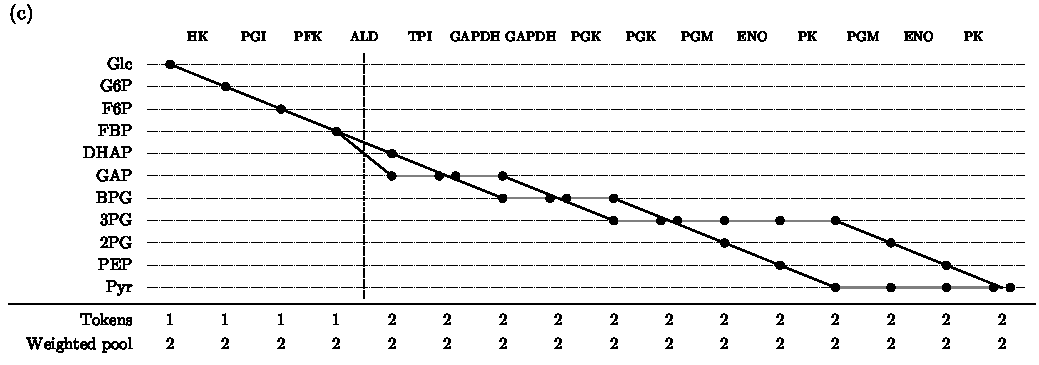
\includegraphics[width=16.4cm]{Figure/glycolysis_replay.pdf}};
\end{tikzpicture}
\endgroup
